%%%%%%%%%%%%%%%%%%%%%%%%%%%%%%%%%%%%%%%%%%%%%%%%%%%%%%%%%%%%%%%
% Welcome to the MAT320 Homework template on Overleaf -- just edit your
% LaTeX on the left, and we'll compile it for you on the right.
%%%%%%%%%%%%%%%%%%%%%%%%%%%%%%%%%%%%%%%%%%%%%%%%%%%%%%%%%%%%%%%
% --------------------------------------------------------------
% Based on a homework template by Dana Ernst.
% --------------------------------------------------------------
% This is all preamble stuff that you don't have to worry about.
% Head down to where it says "Start here"
% --------------------------------------------------------------

\documentclass[12pt]{article}

\usepackage{graphicx}
\graphicspath{{./images/}}
\usepackage[margin=1in]{geometry} 
\usepackage{amsmath,amsthm,amssymb}
% https://tex.stackexchange.com/questions/146306/how-to-make-horizontal-lists
\usepackage[inline]{enumitem} % allows using letters in enumerate list environment

% source: https://stackoverflow.com/questions/3175105/inserting-code-in-this-latex-document-with-indentation

\usepackage{listings}
\usepackage{color}

\definecolor{dkgreen}{rgb}{0,0.6,0}
\definecolor{gray}{rgb}{0.5,0.5,0.5}
\definecolor{mauve}{rgb}{0.58,0,0.82}

\lstset{frame=tb,
	language=C, % language for code listing
	aboveskip=3mm,
	belowskip=3mm,
	showstringspaces=false,
	columns=flexible,
	basicstyle={\small\ttfamily},
	numbers=none,
	numberstyle=\tiny\color{gray},
	keywordstyle=\color{blue},
	commentstyle=\color{dkgreen},
	stringstyle=\color{mauve},
	breaklines=true,
	breakatwhitespace=true,
	tabsize=4
}

\newcommand{\N}{\mathbb{N}}
\newcommand{\Z}{\mathbb{Z}}

\newenvironment{ex}[2][Exercise]{\begin{trivlist}
		\item[\hskip \labelsep {\bfseries #1}\hskip \labelsep {\bfseries #2.}]}{\end{trivlist}}

\newenvironment{sol}[1][Solution]{\begin{trivlist}
		\item[\hskip \labelsep {\bfseries #1:}]}{\end{trivlist}}


\begin{document}

% --------------------------------------------------------------
%                         Start here
% --------------------------------------------------------------

\noindent Sergio Garcia Tapia \hfill

\noindent{\small Concrete Mathematics, by Graham, Knuth, and Patashnik} \hfill 

\noindent{\small Chapter 1: Recurrent Problems} \hfill 

\noindent\today
\subsection*{Warmups}
\begin{ex}{1}
	All horses are the same color; we can prove this by induction on the number
	of horses in a given set. Here's how: ``If there's just one horse then it's the
	same color as itself, so the basis is trivial. For the induction step,
	assume that there are $n$ horses numbered $1$ to $n$. By the induction
	hypothesis, horses 1 through $n-1$ are the same color, and similarly,
	horses 2 through $n$ are the same color. But the middle horses, 2 through $n-1$,
	can't change color when they're in different groups; these are horses, not
	chameleons. So horses 1 and $n$ must be the same color as well, by transitivity.
	Thus all $n$ horses are the same color; QED." What, if anything, is wrong with this
	reasoning?
\end{ex}

\begin{sol}
	It's incorrect because it assumes that the first group of horses numbered
	1 through $n-1$ overlaps with the second group numbered 2 through $n$.
	However, if $n=2$, this corresponds to the groups 1 through 1 and 2 through 2,
	which do not overlap.
\end{sol}

\begin{ex}{2}
	Find the shortest sequence of moves that transfers a tower of $n$ disks
	from the left peg A to the right peg B, if direct moves between A and B
	are disallowed (Each move must be to or from the middle peg. As usual,
	a larger disk must never appear before a smaller one).
\end{ex}

\begin{sol}
	Let $T_n$ be the minimum number of moves that will transfer $n$ disks
	from one peg to another under the given rules. Note that $T_0=0$, $T_1=2$,
	$T_2=8$. For three disks, we the pattern emerges:
	\begin{enumerate}
		\item  We cannot move disk 3 until disks 1 and 2 are both in peg B, so
		first we use $T_2$ moves to do that.
		\item Move disk 3 from A to C.
		\item Move disks 1 and 2 from B to A by going through C; this is $T_2$.
		\item Move disk 3 from C to B.
		\item Move disks 1 and 2 from A to B by going through C; this is $T_2$.
	\end{enumerate}
	In other words, $T_3=2+3T_2$. Generalizing this strategy, we find that
	we can transfer $n$ disks in at most $2+3T_{n-1}$ moves:
	\[
	T_n\leq 2+3T_{n-1},\quad n>0
	\]
	To prove that equality holds, suppose we have $n$ disks. To move the largest disk, disk $n$, we must transfer the $n-1$ smallest onto a single peg. If they are in peg C, we still cannot move the largest disk because transfer from A to B are disallowed. Therefore,
	they must be in B. But this takes precisely $T_{n-1}$ moves. At this point, we transfer
	the largest disk to C. By the same logic, we cannot move the largest disk to C
	until the $n-1$ smallest ones are in a single peg, namely peg A. That takes another
	$T_{n-1}$ moves. Now the single transfer from C to B places the largest disk at its final
	position. Now the $n-1$ smallest disks are in peg A. Moving them to B requires
	another $T_{n-1}$ moves. Hence, the recurrence is:
	\begin{align*}
		T_0&=0;\\
		T_{n}&=3T_{n-1}+2,\quad \text{for } n>0
	\end{align*}
	Let's add 1 to both sides to get:
	\begin{align*}
		T_0+1&=1;\\
		T_n+1&=3T_{n-1}+3,\quad \text{for } n>0
	\end{align*}
	We can substitute $U_{n}=T_{n}+1$ to get
	\begin{align*}
		U_{0}&=1;\\
		U_{n}&=3U_{n-1},\quad \text{for } n>0
	\end{align*}
	The solution is $U_{n}=3^n$, and hence, $T_n=3^{n}-1$.
\end{sol}

\begin{ex}{3}
	Show that, in the process of transferring a tower under the
	restrictions of the preceding exercise, we will actually encounter every properly
	stacked arrangement of $n$ disks on three pegs.
\end{ex}

\begin{sol}
	\begin{proof}
		Let $S_n$ be the number of properly stacked arrangements of $n$ disks on
		the three pegs. The disks begin with a proper arrangement. If a single move
		is made according to the rules of the previous exercise, then the resulting
		arrangement is properly stacked. Moreover, it is a \emph{new} arrangement, for
		if it was an arrangement that we have already seen, then we would be stuck
		in an endless cycle and never be able to ensure the stack of disks lies
		entirely on peg $B$. However, we saw in the previous exercise that it is
		indeed possible to move them to B after $3^n-1$ moves. Therefore, each move gives rise
		to a new arrangement, suggesting that
		\[
		T_n+1\leq S_n
		\]
		where $T_n=3^n-1$ as in the previous exercise, and the $+1$ accounts for
		the initial arrangement. Label each disk with an integer from $\{1,\ldots, n\}$,
		and let $D_A$, $D_B$, and $D_C$ denote the set of disks in each of pegs $A$,
		$B$, and $C$, respectively:
		\begin{enumerate}
			\item $D_A$ corresponds to a subset of $\{1, \ldots, n\}$: This follows
			because the only way to stack disks on a peg is from largest to smallest.
			The same is true for $D_B$ and $D_C$.
			\item $D_A$, $D_B$, and $D_C$ are disjoint: no two pegs contain the
			same disk.
			\item $D_A\cup D_B\cup D_C=\{1,\ldots,n\}$: Every disk is in one
			of the three pegs.
		\end{enumerate}
		In other words, $D_A$, $D_B$, and $D_C$ partition $\{1,\ldots, n\}$. The
		number of arrangements is then equivalent to the number of such partitions.
		Next, we prove that the number of such partition is $3^n$. The basis holds
		because if $n=1$, we have:
		\begin{enumerate}
			\item $D_A=\{1\}, D_B=\emptyset, D_C=\emptyset$
			\item $D_A=\emptyset, D_B=\{1\}, D_C=\emptyset$
			\item $D_A=\emptyset, D_B=\emptyset, D_C=\{1\}$
		\end{enumerate}
		which is $3=3^1$. Suppose that every set of $n-1$ elements has $3^{n-1}$
		partitions, for $n>1$. Suppose we have a set of $n$ elements.
		If $1\leq k\leq n$, let $Y_k$ be the set obtained by removing $k$
		from $\{1,\ldots, n\}$. Then $Y_k$ has $n-1$ elements, and it can be
		partitioned into three distinct subsets in $3^{n-1}$ distinct ways.
		Suppose the 3 subsets are called $D_A, D_B, D_C$. By adding $k$
		to any one of them, we obtain a partition of $\{1, \ldots, n\}$ into
		three sets, one of:
		\begin{enumerate}
			\item $(D_A\cup\{k\}, D_B, D_C)$
			\item $(D_A, D_B\cup\{k\}, D_C)$
			\item $(D_A, D_B, D_C\cup\{k\})$
		\end{enumerate}
		Since we have 3 choices for each partition of $Y_k$, it follows that
		the number of partitions of $\{1,\ldots,n\}$ is $3\cdot 3^{n-1}=3^n$.
		We have now proved that $S_n=3^{n}$, thus, that every arrangement is
		reachable via a transfer as described in the previous exercise.
	\end{proof}
\end{sol}

\begin{ex}{4}
	Are there any starting and ending configurations of $n$ disks on three
	pegs that are more than $2^{n}-1$ moves apart, under Lucas's original rules?
\end{ex}

\begin{sol}
	No. The maximum number of moves between two configurations is $2^{n-1}$. For the basis,
	$n_1$, we have 3 configurations, and they are all reachable with 1 move.
	For the inductive hypothesis, assume $n>1$, we know that $n-1$ disks
	are at most $2^{n-1}-1$ moves apart. Suppose we have a starting and ending configuration
	of $n$ disks. For both, the smallest disk is the topmost disk on one of the pegs.
	Consider the modified start and end configurations without the smallest disk.
	If the smallest disk were not present, then at most $2^{n-1}-1$ moves would bring us
	to the end configuration. If before each move we had to move the smallest out of the
	way, then we might need twice as many moves, or $2(2^{n-1}-1)=2^n-2$. We might
	require one last move to place the smallest disk in the desired place, 
	for a maximum of $2^{n}-2+1=2^{n}-1$ moves.
\end{sol}

\begin{ex}{5}
	A ``Venn diagram" with three overlapping circles is often used to illustrate
	the eight possible subsets associated with three given sets:
	\begin{center}
		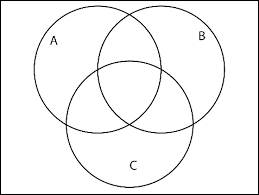
\includegraphics[width=0.3\textwidth]{venn-diagram-3-sets}
	\end{center}
	Can the sixteen possibilities that arise with four given sets be illustrated
	by four overlapping circles?
\end{ex}

\begin{sol}
	The 8 sets in questions are given below.
	\begin{center}
		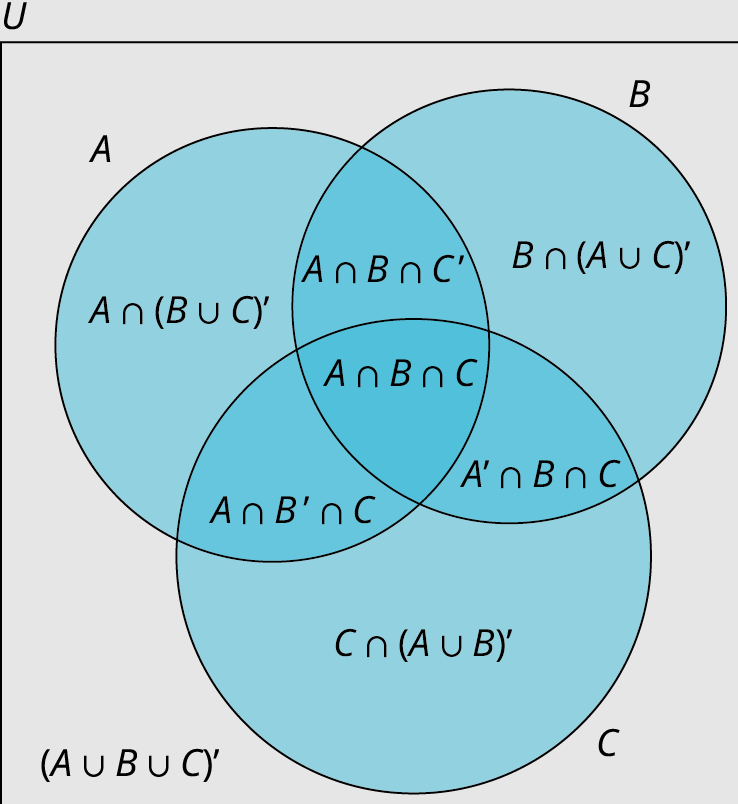
\includegraphics[width=0.3\textwidth]{venn-diagram-3-sets-8-subsets}
	\end{center}
	The necessary 16 sets cannot be illustrated by four overlapping circles.
	Note that any pair of circles intersects in at most 2 points
	Each intersection increases the number of regions by 1. Therefore, when
	a fourth circle is added to the Venn diagram above, we get at most 6 intersections (2
	for each of the 3 circles), and hence at most 14 regions exist.
\end{sol}

\begin{ex}{6}
	Some of the regions defined by $n$ lines in the plane are infinite, while others
	are bounded. What's the maximum possible number of bounded regions?
\end{ex}

\begin{sol}
	Note that any bounded region created from intersecting lines has at least 3 vertices.
	Let $B_n$ be the number of bounded regions defined by $n$ lines in the plane.
	Since we need at least 3 vertices, $B_0=0$, $B_1=0$, $B_2=0$. Starting with $n=3$,
	choosing a non-parallel line, it intersects in 2points (1 for each existing line).
	It creates a single, triangular region, therefore $B_3=3$. A fourth line intersects
	the remaining 3 in 3 points. If the line intersects the two lines of a bounded
	region, it splits that region in 2, adding one new region. If, instead,
	the two lines being intersected define an unbounded region, the intersection
	creates a new bounded region. Either way, a new region is created.
	Hence, the intersection with $3$ points results in 2 new regions. This also serves
	as a proof by induction. Therefore,
	\begin{align*}
		B_0&=0\\
		B_1&=0\\
		B_2&=0\\
		B_{n}&=S_{n-2},\quad n>2
	\end{align*}
	where $S_n$ is the triangular number $n(n+1)/2$.
\end{sol}

\begin{ex}{7}
	Let $H(n)=J(n+1)-J(n)$. Equation (1.8) tells us that $H(2n)=2$, and
	$H(2n+1)=J(2n+2)-J(2n+1)=(2J(n+1)-1)-(2J(n)+1)=2H(n)-2$, for all $n\geq 1$.
	Therefore it seems possible to prove that $H(n)=2$ for all $n$, by induction
	on $n$. What's wrong here?
\end{ex}

\begin{sol}
	The basis is not true, since
	\[
	H(1)=J(2)-J(1)=2J(1)-1-J(1)=J(1)-1=1-1=0.
	\]
\end{sol}

\subsection*{Homework exercises}
\begin{ex}{8}
	Solve the recurrence 
	\begin{align*}
		Q_0&=\alpha;\quad Q_1=\beta;\\
		Q_n&=(1+Q_{n-1})/Q_{n-2},\quad \text{for } n>1.
	\end{align*}
	Assume that $Q_n\neq 0$ for all $n\geq 0$. \emph{Hint}: $Q_4=(1+\alpha)/\beta$.
\end{ex}

\begin{sol}
	\begin{proof}
		Computing a few values, we find:
		\begin{align*}
			Q_2&=\frac{1+\beta}{\alpha}\\
			Q_3&=\frac{1+\frac{1+\beta}{\alpha}}{\beta}\\
			&=\frac{1+\alpha+\beta}{\alpha\beta}\\
			Q_4&=\frac{1+\alpha}{\beta}\\
			Q_5&=\frac{1+\frac{1+\alpha}{\beta}}{\frac{1+\alpha+\beta}{\alpha\beta}}\\
			&=\alpha\\
			Q_6&=\frac{1+\alpha}{\frac{1+\alpha}{\beta}}\\
			&=\beta
		\end{align*}
		Note that $Q_5=Q_0$ and $Q_6=Q_1$. Since $Q_n$ for $n>1$ is given
		in terms of the previous two terms, this implies that $Q_n$ is cyclic with
		a period of 5, meaning that $Q_{n}=Q_{n-5}$ for all $n\geq 5$. Hence, the solution
		is
		\begin{align*}
			Q_0&=\alpha\\
			Q_1&=\beta\\
			Q_2&=\frac{1+\beta}{\alpha}\\
			Q_3&=\frac{1+\alpha+\beta}{\alpha\beta}\\
			Q_4&=\frac{1+\alpha}{\beta}\\
			Q_{n}&=Q_{n-5},\quad \text{for } n \geq 5
		\end{align*}
	\end{proof}
\end{sol}

\begin{ex}{9}
	Sometimes it's possible to use induction backwards, proving things from
	$n$ to $n-1$ instead of vice versa! For example, consider the statement
	\[
	P(n):\quad x_1\cdots x_n\leq \left(\frac{x_1+\cdots+x_n}{n}\right)^n,\quad
	\text{if } x_1,\ldots,x_n\geq 0.
	\]
	This is true when $n=2$ since $(x_1+x_2)^2-4x_1x_2=(x_1-x_2)^2\geq 0$.
	\begin{enumerate}[label=(\alph*)]
		\item By setting $x_n=(x_1+\cdots+x_{n-1})/(n-1)$, prove that $P(n)$
		implies $P(n-1)$ whenever $n>1$.
		\item Show that $P(n)$ and $P(2)$ imply $P(2n)$.
		\item Explain why this implies the truth of $P(n)$ for all $n$.
	\end{enumerate}
\end{ex}

\begin{sol}
	\
	\begin{enumerate}[label=(\alph*)]
		\item \begin{proof}
			If all $x_i$ are 0, then the statement is definitely true.
			Suppose that at least one $x_i$ is nonzero, and that $P(n)$ holds.
			Setting $x_n=(x_1+\cdots+x_{n-1})/(n-1)$, we find
			\begin{align*}
				x_1\cdots x_{n-1}\cdot \left(\frac{x_1+\cdots+x_{n-1}}{n-1}\right)
				&\leq
				\left(\frac{x_1+\cdots+x_{n-1}+
				\left(\frac{x_1+\cdots+x_{n-1}}{n-1}\right)
				}{n}\right)^n\\
				&\leq \left(
				\frac{
					\frac{(n-1)x_1+\cdots+(n-1)x_{n-1}+x_1+\cdots+x_{n-1}}{n-1}
				}{n}
				\right)^n\\
				&\leq \left(
				\frac{x_1+\cdots+x_{n-1}}{n-1}
				\right)^n
			\end{align*}
			Since both sides have a factor of $(x_1+\cdots+x_{n-1})/(n-1)$, and since
			at least one $x_i$ is nonzero, the term is positive, so we can divide by it
			without changing the inequality direction:
			\begin{align*}
				x_1\cdots x_{n-1}\leq \left(\frac{x_1+\cdots+x_{n-1}}{n-1}\right)^{n-1}
			\end{align*}
			This is precisely $P(n-1)$.
		\end{proof}
		\item \begin{proof}
			We were given that $P(2)$ is true. Suppose $P(n)$ is also true. Then
			\begin{align*}
				x_1x_2\cdots x_{2n-1}x_{2n}	&=(x_1x_2)\cdots (x_{2n-1}x_{2n})\\
				&\leq
				\left(\frac{x_1+x_2}{2}\right)^2\cdots \left(\frac{x_{2n-1}+x_{2n}}{2}\right)^2
				\qquad\text{(By $P(2)$)}\\
				&=
				\left(
				\frac{1}{2}
				\right)^{2n}
				(x_1+x_2)^2\cdots (x_{2n-1}+x_{2n})^2\\
				&=\left(
				\frac{1}{2}
				\right)^{2n}
				\left((x_1+x_2)\cdots (x_{2n-1}+x_{2n})\right)^2\\
				&\leq\left(
				\frac{1}{2}
				\right)^{2n}
				\left(
				\frac{(x_1+x_2)+\cdots +(x_{2n-1}+x_{2n})}{n}
				\right)^{2n}\qquad\text{(By $P(n)$)}\\
				&=\left(
				\frac{x_1+\cdots+x_{2n}}{2n}
				\right)^{2n}
			\end{align*}
			
		\end{proof}
		\item We know it holds for $P(2)$. Suppose that $n>2$, and that it holds for
		$2$ through $n-1$.
		\begin{enumerate}[label=(\roman*)]
			\item If $n$ is even, then $n=2k$, and since $2\leq k\leq n-1$,
			it holds for $P(k)$ by induction, so it must hold for $P(2k)=P(n)$ (since it holds
			for $P(2)$) by (b).
			\item If $n$ is odd, then $n=2k-1$ for some $k>1$. Since $n\geq 3$, it
			follows that $k=\frac{n+1}{2}\leq n-1$, so $P(k)$ holds, implying that $P(2k)$ holds
			by (b). Now $P(2k-1)$ holds by (a).
		\end{enumerate}
		The result now holds for all $n$ by induction.
	\end{enumerate}
\end{sol}

\begin{ex}{10}
	Let $Q_n$ be the minimum number of moves needed to transfer a tower of $n$ disks
	from $A$ to $B$ if all moves must be made \emph{clockwise} --- that is, from $A$
	to $B$, or from $B$ to the other peg, or from the other peg to $A$. Also, let
	$R_n$ be the minimum number of moves needed to go from $B$ back to $A$
	under this restriction. Prove that
	\begin{align*}
		Q_n=\begin{cases}
			0, & \text{if } n =0;\\
			2R_{n-1}+1, & \text{if } n>0;
		\end{cases}
		\quad
		R_n=\begin{cases}
			0, & \text{if } n =0;\\
			Q_n+Q_{n-1}+1, & \text{if } n>0.
		\end{cases}
	\end{align*}
	(You need not solve these recurrences; we'll see how to do that in Chapter 7.)
\end{ex}

\begin{sol}
	\begin{proof}
		We begin by proving that
		\[
		Q_n=2R_{n-1}+1
		\]
		\begin{enumerate}[label=(\alph*)]
			\item \emph{Move disks 1 through $n-1$ from $A$ to $C$}: This is necessary
			because we want to move disk $n$ to peg $B$, and that pegs needs to be
			empty since disk $n$ is the largest move. It takes $R_{n-1}$ moves to
			do this.
			\item \emph{Move disk $n$ from $A$ to $B$}: This takes a single move.
			\item \emph{Move disk 1 through $n-1$ from $C$ to $B$}: This takes
			$R_{n-1}$.
		\end{enumerate}
		The moves made were necessary and sufficient, so the equation is proved.
		The hints in Appendix A suggest proceeding by proving that
		\[
		R_n=R_{n-1}+1+Q_{n-1}+1+R_{n-1},\quad n>0
		\]
		Suppose disks $1$ through $n$ are stacked on peg B, and we wish to move
		the stack to peg A. We can do so as follows:
		\begin{enumerate}[label=(\roman*)]
			\item \emph{Move disks 1 through $n-1$ to $A$}: This is necessary because we
			need to eventually move disk $n$ to peg $C$ (before going to $A$). Since it
			is the largest disk, there can be no other disk on peg $C$, and hence every
			disk must be on peg A. This takes $R_{n-1}$ moves.
			\item \emph{Move disk $n$ from B to C}: This takes a single move.
			\item \emph{Move disks 1 through $n-1$ from $A$ to $B$}: In order to have
			disk $n$ on peg A, that peg must be empty, so every disk must be on peg B.
			This will take $Q_{n-1}$ moves.
			\item \emph{Move disk $n$ from $C$ to $A$}: This takes 1 more.
			\item \emph{Move disks $1$ through $n-1$ from $B$ to $A$}: This takes
			$R_{n-1}$.
		\end{enumerate}
		We can combine these to get the desired equation for $R_n$:
		\begin{align*}
			R_{n}&=R_{n-1}+1+Q_{n-1}+1+R_{n-1}\\
			&=(2R_{n-1}+1)+Q_{n-1}+1\\
			&=Q_n+Q_{n-1}+1
		\end{align*}
		as we set out to show.
	\end{proof}
\end{sol}

\begin{ex}{11}
	A Double Tower of Hanoi contains $2n$ disks of $n$ different sizes, two of each size.
	As usual, we're required to move only one disk at a time, without putting a larger one
	over a smaller one.
	\begin{enumerate}[label=(\alph*)]
		\item How many moves does it take to transfer a double tower from one peg to another,
		if disks of equal size are indistinguishable from each other?
		\item What if we required to reproduce the original top-to-bottom
		order of all the equal-size disks in the final arrangement?
		[\emph{Hint}: This is difficult --- it's really a ``bonus problem"].
	\end{enumerate}
\end{ex}

\begin{sol}
	\
	\begin{enumerate}[label=(\alph*)]
		\item Let $S_{n}$ be the number of moves it takes to move the Double Tower of
		Hanoi of $2n$ disks.  If $n=1$, then it takes 2 moves, since the two disks are
		indistinguishable and can be stacked, so $S_{1}=2$. If $n>1$, suppose we start
		with $2n$ disks on peg A. To move the tower to peg B, we do the following:
		\begin{enumerate}[label=(\alph*)]
			\item \emph{Move smallest $2n-2$ disks from A to C}: This is a pre-requisite
			to moving the largest two disks to B. Since B must be empty before placing
			the two largest disks, it follows that every other disk must be in C.
			This takes $S_{n-1}$ moves.
			\item  \emph{Move the two largest disks from A to B}: This takes two moves.
			This flips their order, which is allowed because the disks are indistinguishable,
			and disks of the same size can be stacked.
			\item \emph{Move the remaining disks from C to B}: This takes $S_{n-1}$ moves.
		\end{enumerate}
		Hence, $S_{n}=2S_{n-1}+2$, and $S_1=2$. We can now solve by first adding 2
		to both sides and substituting:
		\begin{align*}
			S_1+2&=4\\
			S_n+2&=2S_{n-1}+4=2(S_{n-1}+2)
		\end{align*}
		Let $T_n=S_{n}+2$. Then the recurrence becomes
		\begin{align*}
			T_1&=4\\
			T_{n}&=2T_n
		\end{align*}
		The solution is $T_n=2\cdot 2^{n}=2^{n+1}$, so $S_n=2^{n+1}-2$.
		\item Let $X_n$ be the minimum number of moves to achieve the goal.
		Then $X_1=3$, since we move the first disk from $A$ to $C$, the second
		disk from $A$ to $B$, and the first disk from $C$ to $A$. Call the two
		largest disks $n$ and $n'$, with $n'$ at the bottom. For
		$n>1$, we do the following:
		\begin{enumerate}[label=(\roman*)]
			\item \emph{Move smallest $2n-2$ disks from $A$ to $B$}: This is necessary
			in order to start moving the largest disks. This takes $S_{n-1}$ moves,
			where $S_n$ is defined in part (a).
			\item \emph{Move disk $n$ from $A$ to $C$}: This takes 1 move.
			\item \emph{Move smallest $2n-2$ disks from $B$ to $C$}: Since we cannot
			put $n'$ on top of $n$ (which would flip the disks), we need $n$ on
			peg $B$, and hence, that disk must be empty. This takes $S_{n-1}$ moves.
			\item \emph{Move disk $n$ from $A$ to $B$}: This takes 1 move.
			\item \emph{Move smallest $2n-2$ disks from $C$ to $A$}: This is required
			to move disk $n$ on top of $n'$. This takes $S_{n-1}$ moves.
			\item \emph{Move $n$ from $C$ to $B$}: This takes 1 move. Now $n$ is
			on top of $n'$ just like at the start, but they're on peg B.
			\item \emph{Move smallest $2n-2$ disks from $A$ to $B$}: This takes $2n-2$ moves.
		\end{enumerate}
		At this point, we'll have moved the stack of $2n-2$ disks a total of 4 times,
		so it is back in its original arrangement. Hence,
		\[
		X_n=4S_{n-1}+3=4(2^{n}-2)+3=2^{n+2}-8+3=2^{n+2}-5
		\]
	\end{enumerate}
\end{sol}

\begin{ex}{12}
	Let's generalize exercise 11a even further, by assuming that there are $n$ different
	sizes of disks and exactly $m_k$ disks of size $k$. Determine $A(m_1, \ldots, m_n)$,
	the minimum number of moves needed to transfer a tower when equal-size disks are
	considered indistinguishable.
\end{ex}

\begin{sol}
	If $n=1$, then $A(m_1)=m_1$. Suppose $n>1$, and $m_k>0$ each $k$. Suppose
	all disks start on peg $A$ and want to transfer all disks to $B$::
	\begin{enumerate}[label=(\alph*)]
		\item \emph{Move all disks of sizes $1,\ldots,n-1$ to $C$}: This
		is required to be able to move the disks of size $m_n$. This takes
		$A(m_1,\ldots, m_{n-1})$ moves.
		\item \emph{Move all disks of size $n$}: This takes $m_n$ moves since
		there are $m_n$ such disks.
		\item \emph{Move all disks of size $1,\ldots, n-2$ to $B$}: This takes
		$A(m_1,\ldots, m_{n-1})$ moves again.
	\end{enumerate}
	Hence, $A(m_1,\ldots, m_n)=2A(m_1,\ldots,m_{n-1})+m_n$, which we can unfold as follows:
	\begin{align*}
		A(m_1,\ldots, m_n)&=2A(m_1,\ldots,m_{n-1})+m_n\\
		&=4A(m_1,\ldots, m_{n-2})+2m_{n-1}+m_n\\
		&=2^{n-1}A(m_1)+2^{n-2}m_2+\cdots+2m_{n-1}+m_n\\
		&=2^{n-1}m_1+2^{n-2}m_2+\cdots+2m_{n-1}+m_n
	\end{align*}
\end{sol}

\begin{ex}{13}
	What's the maximum number of regions definable by $n$ zig-zag lines,
	each of which consists of two parallel infinite half-lines joined by
	a straight segment? Given: $ZZ_2=12$.
\end{ex}

\begin{sol}
	Note $ZZ_1=2$, and we are given that $ZZ_2=12$. There are 2 unbounded regions
	and 0 bounded regions for $ZZ_1$, and there are 4 unbounded regions and 8
	bounded regions for $ZZ_2$. Moreover, there are 9 intersection points between
	the two zig-zags. Let's consider $ZZ_3$.
	\
	
	For $ZZ_3$, we get 2 new unbounded regions, and since there are 2 existing
	zig-zag lines, the new one intersects each of those in 9 points, and hence,
	a total of 18 points, so it should create 17 new bounded regions.
	That is, altogether, we have 19 new regions, so the new total should be 31.
	
	For the general case, suppose we have $ZZ_{n-1}$ regions with $n-1$ zig-zag lines. If we ensure the $n$th zig-zag intersects every other zig-zag in 9
	intersection points, then we will add 2 unbounded regions (due to each infinite
	segment of the new zig-zag) and if there are $k$ intersections, we get $k-1$
	bounded regions. We can ensure the new zig-zag intersects every other
	zig-zag in 9 points, for a total of $9(n-1)$ new intersections, which
	creates $9(n-1)-1$ new regions. Hence:
	\[
	ZZ_n=ZZ_{n-1}+9(n-1)-1+2
	\]
	We can unfold it to get the closed:
	\begin{align*}
		ZZ_n&=Z_1+9(1+\cdots+n-1)+2\cdot (n-1)-1(n-1)\\
		&=Z_1+9\cdot \frac{(n-1)n}{2}+n-1\\
		&=Z_1+\frac{9}{2}n^2-\frac{9}{2}n+n-1\\
		&=\frac{9}{2}n^2-\frac{7}{2}n+1
	\end{align*}
\end{sol}

\begin{ex}{14}
	How many pieces of cheese can you obtain from a single thick piece
	by making five straight slices? (The cheese must stay in its original
	position while you do all the cutting, and each slice must correspond
	to a plane in 3D). Find a recurrence relation for $P_n$, the maximum
	number of three-dimensional regions that can be defined by $n$
	different planes.
\end{ex}

\begin{ex}{15}
	Josephus had a friend who was saved by getting into the next-to-last
	position. What is $I(n)$, the number of the penultimate survivor when
	every second person is executed?
\end{ex}

\begin{sol}
	Note if there are 10 people, the survivor is 5, but the penultimate survivor
	is 9, so $I(10)=9$. The following table shows some values:
	\begin{center}
		\begin{tabular}{c|c|ccc|cccccc|c}
			$n$    & 2 & 3 & 4 & 5 & 6 & 7 & 8 & 9 & 10 &  11 & 12\\
			\hline
			$I(n)$ & 2 & 1 & 3 & 5 & 1 & 3 & 5 & 7 & 9  &  11 & 1
		\end{tabular}
	\end{center}
	Notice that $I(1)$ is not defined. An analysis similar to the Josephus
	problem leads to:
	\begin{align*}
		I(2)&=2;\\
		I(3)&=1;\\
		I(2n)&=2I(n)-1,\quad n\geq 2,\\
		I(2n+1)&=2I(n)+1,\quad n\geq 2
	\end{align*}
	The sample of table values show that when $n=3\cdot 2^{m}$,
	we have $I(n)=1$, marking the start of an increasing group of odd
	numbers. The next group starts at $3\cdot 2^{m+1}$, and $I(3\cdot 2^{m+1})=1$
	The number of values in each group is
	$3\cdot 2^{m+1}-3\cdot 2^{m}=3\cdot 2^{m}$. Therefore, we can write
	$n$ as the start of each group plus an offset. That is, we can write
	$n=3\cdot 2^{m}+l$, for some $m\geq 0$ and $0\leq l < 3\cdot 2^{m}$.
	Then
	\[
	I(n)=I(3\cdot 2^{m}+l)=2l+1,\quad m\geq 0 \text{ and } 0\leq l< 3\cdot 2^{m}
	\]
	We proceed by induction on $m$. When $m=0$, we see that $l=0$, giving
	$I(3)=2\cdot 0 + 1=1$, which is true. For the induction step, first
	consider the case when $3\cdot 2^{m}+l$ is even. This implies that
	$l$ is even, so
	\begin{align*}
		I(3\cdot 2^m + l)=2I(2^{m-1}+l/2)-1=2(2l/2 + 1)-1=2l+1
	\end{align*}
	The odd case is similar, using $I(2n+1)$ instead. The equation holds
	for all $n$.
\end{sol}

\begin{ex}{16}
	Use the repertoire method to solve the general four-parameter recurrence
	\begin{align*}
		g(1)&=\alpha;\\
		g(2n+j)&=3g(n)+\gamma n+\beta_j,\quad \text{for } j=0,1,\text{ and } n\geq 1
	\end{align*}
	\emph{Hint}: Try the function $g(n)=n$.
\end{ex}

\begin{sol}
	Let us suppose that the solution has the form
	\[
	g(n)=A(n)\alpha+B(n)\beta_0+C(n)\beta_1+D(n)\gamma
	\]
	First let's suppose $g(n)=n$. Then
	\begin{align*}
		1 &= \alpha\\
		2n &= 3n + \beta_0\quad\implies\quad -n=\beta_0\\
		2n + 1 &= 3n + \gamma n + \beta_1\quad\implies\quad -n+1=\gamma_n+\beta_1
	\end{align*}
	
	By treating the equations as polynomials in $n$ and equating coefficients,
	we conclude that $\alpha=1$, $\beta_0=0$, $\beta_1=1$, and $\gamma=-1$.
	Now let $g(1)=1$. We get the equations
	\begin{align*}
		1&=\alpha\\
		1&=3+\gamma n+\beta_0\\
		1&^=3+\gamma n+\beta_1
	\end{align*}
	Similar to before, we conclude that $\alpha=1$, $\beta_0=\beta_1=-2$, and $\gamma=0$.
	Hence, we get the equations:
	\begin{align*}
		A(n)+C(n)-D(n)&=n\\
		A(n)-2B(n)-2C(n)&=1
	\end{align*}
	We can solve by determining two of the functions, and expressing
	the remaining two in terms of those. For example, if we
	set $\alpha=1$ and $\gamma=\beta_0=\beta_1=0$, then
	$g(n)=A(n)$, and
	\begin{align*}
		A(1)&=1\\
		A(2n)&=3A(n)\\
		A(2n+1)&=3A(n)
	\end{align*}
	Creating a table reveals that if we let $n=2^{m}+l$, where $m\geq 0$
	and $0\leq l<m$, then $A(2^m+l)=3^m$. We could do this for one more
	function to and be done. Alternatively, as pointed out in the Appendix
	for the solution to this problem, setting $\gamma=0$ leaves us with
	\begin{align*}
		g(1)&=\alpha\\
		g(2n+j)&=3g(n)+\beta_j,\quad 0\leq j<1 \text{ and } n\geq1
	\end{align*}
	Therefore, this defines $A(n)\alpha+B(n)\beta_0+C(n)\beta_1$ to be
	the radix-changing function, from radix 2 to radix 3. Namely, converting $n=(1b_{m-1}b_{m-2}\ldots b_1b_0)_2$ to $(\alpha\beta_{b_{m-1}}\beta_{b_{m-2}}\ldots \beta_{b_0})_3$. In othet words, $A(n)$, $B(n)$, and $C(n)$ are determined
	when $\gamma=0$, and we can express $D(n)$ in terms of them.
	Hence, all functions are determined.
\end{sol}

\end{document}